%%%%%%%%%% format 2012/2/3 %%%%%%%%%%%%
\documentclass[titlepage,twoside]{jarticle}
\usepackage{latexsym}
\usepackage{amsmath}
\usepackage{amssymb}
\usepackage{amsthm}
\theoremstyle{definition}
\newtheorem{thm}{定理}
\usepackage{listings}
\usepackage{bm}

\usepackage[dvipdfmx]{graphicx}
\usepackage{url}
\usepackage{fancybox}

%Windows, Mac, Unixで栞が文字化けしないように自動判別+hyperrefの設定.
\ifx\kanjiskip\undefined\else %platexやjlatexなどで処理する場合ということ
  \usepackage{atbegshi}
  \ifx\ucs\undefined
    \ifnum 42146=\euc"A4A2
      \AtBeginShipoutFirst{\special{pdf:tounicode EUC-UCS2}}
    \else
      \AtBeginShipoutFirst{\special{pdf:tounicode 90ms-RKSJ-UCS2}}
    \fi
  \else
    \AtBeginShipoutFirst{\special{pdf:tounicode UTF8-UTF16}}
  \fi
  \usepackage[dvipdfmx,bookmarks=true,bookmarksnumbered=true,%
  %bookmarkstype=toc,colorlinks=true,linktocpage=true]{hyperref}
  bookmarkstype=toc]{hyperref}
\fi



\setlength{\oddsidemargin}{0.5cm}
\setlength{\evensidemargin}{-0.5cm}
\setlength{\topmargin}{-1cm}
\setlength{\textwidth}{15.5cm}
\setlength{\textheight}{21.5cm}

\ifx\kanjiskip\undefined\else %platexやjlatexなどで処理する場合ということ
\DeclareRelationFont{JY1}{mc}{it}{}{OT1}{cmr}{it}{}
\DeclareRelationFont{JT1}{mc}{it}{}{OT1}{cmr}{it}{}
\DeclareFontShape{JY1}{mc}{m}{it}{<5> <6> <7> <8> <9> <10> sgen*min
    <10.95><12><14.4><17.28><20.74><24.88> min10
    <-> min10}{}
\DeclareFontShape{JT1}{mc}{m}{it}{<5> <6> <7> <8> <9> <10> sgen*tmin
    <10.95><12><14.4><17.28><20.74><24.88> tmin10
    <-> tmin10}{}
\DeclareRelationFont{JY1}{mc}{sl}{}{OT1}{cmr}{sl}{}
\DeclareRelationFont{JT1}{mc}{sl}{}{OT1}{cmr}{sl}{}
\DeclareFontShape{JY1}{mc}{m}{sl}{<5> <6> <7> <8> <9> <10> sgen*min
    <10.95><12><14.4><17.28><20.74><24.88> min10
    <-> min10}{}
\DeclareFontShape{JT1}{mc}{m}{sl}{<5> <6> <7> <8> <9> <10> sgen*tmin
    <10.95><12><14.4><17.28><20.74><24.88> tmin10
    <-> tmin10}{}
\DeclareRelationFont{JY1}{mc}{sc}{}{OT1}{cmr}{sc}{}
\DeclareRelationFont{JT1}{mc}{sc}{}{OT1}{cmr}{sc}{}
\DeclareFontShape{JY1}{mc}{m}{sc}{<5> <6> <7> <8> <9> <10> sgen*min
    <10.95><12><14.4><17.28><20.74><24.88> min10
    <-> min10}{}
\DeclareFontShape{JT1}{mc}{m}{sc}{<5> <6> <7> <8> <9> <10> sgen*tmin
    <10.95><12><14.4><17.28><20.74><24.88> tmin10
    <-> tmin10}{}
\DeclareRelationFont{JY1}{gt}{it}{}{OT1}{cmbx}{it}{}
\DeclareRelationFont{JT1}{gt}{it}{}{OT1}{cmbx}{it}{}
\DeclareFontShape{JY1}{mc}{bx}{it}{<5> <6> <7> <8> <9> <10> sgen*goth
    <10.95><12><14.4><17.28><20.74><24.88> goth10
    <-> goth10}{}
\DeclareFontShape{JT1}{mc}{bx}{it}{<5> <6> <7> <8> <9> <10> sgen*tgoth
    <10.95><12><14.4><17.28><20.74><24.88> tgoth10
    <-> tgoth10}{}
\DeclareRelationFont{JY1}{gt}{sl}{}{OT1}{cmbx}{sl}{}
\DeclareRelationFont{JT1}{gt}{sl}{}{OT1}{cmbx}{sl}{}
\DeclareFontShape{JY1}{mc}{bx}{sl}{<5> <6> <7> <8> <9> <10> sgen*goth
    <10.95><12><14.4><17.28><20.74><24.88> goth10
    <-> goth10}{}
\DeclareFontShape{JT1}{mc}{bx}{sl}{<5> <6> <7> <8> <9> <10> sgen*tgoth
    <10.95><12><14.4><17.28><20.74><24.88> tgoth10
    <-> tgoth10}{}
\DeclareRelationFont{JY1}{gt}{sc}{}{OT1}{cmbx}{sc}{}
\DeclareRelationFont{JT1}{gt}{sc}{}{OT1}{cmbx}{sc}{}
\DeclareFontShape{JY1}{mc}{bx}{sc}{<5> <6> <7> <8> <9> <10> sgen*goth
    <10.95><12><14.4><17.28><20.74><24.88> goth10
    <-> goth10}{}
\DeclareFontShape{JT1}{mc}{bx}{sc}{<5> <6> <7> <8> <9> <10> sgen*tgoth
    <10.95><12><14.4><17.28><20.74><24.88> tgoth10
    <-> tgoth10}{}
\DeclareRelationFont{JY1}{gt}{it}{}{OT1}{cmr}{it}{}
\DeclareRelationFont{JT1}{gt}{it}{}{OT1}{cmr}{it}{}
\DeclareFontShape{JY1}{gt}{m}{it}{<5> <6> <7> <8> <9> <10> sgen*goth
    <10.95><12><14.4><17.28><20.74><24.88> goth10
    <-> goth10}{}
\DeclareFontShape{JT1}{gt}{m}{it}{<5> <6> <7> <8> <9> <10> sgen*tgoth
    <10.95><12><14.4><17.28><20.74><24.88> tgoth10
    <-> tgoth10}{}
\fi
%%%% end of jdummy.def

\begin{document}
\title{{\Huge 無情報事前分布によるLomax分布のパラメータ推定}}
\author{\vspace*{50mm}\ \\理学部 応用数学科\\ 学籍番号 1418112 氏名 三國 憲太郎}
\date{}

\maketitle
\newpage
\tableofcontents
\newpage
\section{はじめに}

Lomax 分布は Pareto Type II 分布とも呼ばれ, 経済や保険などに用いられることが多い. データが裾の重い分布に従うと考えられるときは指数分布の代わりにLomax分布を使うことが望ましい.

本論文では\cite{Lomax2020}を元に実際にシミュレーションを実行し,その方法やパフォーマンスについて検討する。ベイズ推定を行う上で, 事後分布が確率の公理を満たさないこと(improperとなること)は望ましくない. ここでは$2$つの無情報事前分布を考え, それぞれに対する事後分布が確率の公理を満たすかどうか(properとなるかどうか)を確認する. 推定のパフォーマンスを確認するために最尤法と比較したシミュレーションを行う. MRE(平均相対誤差)とMSE(平均二乗誤差)により推定の精度を評価する.

\section{ベイズ理論}

\subsection{ベイズ推定}

ベイズ推定は推定するパラメータを確率変数として考える手法である. パラメータに関する事前の知識から事前分布を決め, 観測されたデータを用いて事後分布を計算する. 求めるパラメータを$\theta$, 事前分布を$p(\theta)$とする. $\bm{x}$を観測データとすると事後分布$p(\theta|\bm{x})$はベイズの定理を用いて
$$
p(\theta|\bm{x}) = \dfrac{p(\bm{x}|\theta)p(\theta)}{p(\bm{x})}
$$
と表される. 通常, 事後分布は複雑な形になりそのまま扱うことが困難であることが多いため, 事後分布に従う乱数を生成して評価する. 本論文ではメトロポリス法~(\ref{metropolis}節参照)を用いて事後分布に従う乱数を生成する.

事後分布が
$$
\int_{-\infty}^{\infty}p(\theta|\bm{x})d\theta \neq 1
$$
となり, 確率の公理を満たさなくなる場合がある. このような事後分布をimproperな事後分布という. 事後分布が確率の公理を満たさない状態は望ましくない. これについて\ref{prior}章で詳しく扱う. 

事前分布はパラメータに関する事前情報から決めるが, 事前情報がない場合には無情報事前分布を用いる. 本論文では無情報事前分布の一つであるJeffreysの事前分布(\ref{Jeffreys prior})と, パラメータ間の事前独立性を仮定したJeffreysの事前分布(\ref{independent prior})を考える.

\subsection{メトロポリス法}\label{metropolis}

この章の参考文献は\cite{wakui}である. ベイズ統計では事後分布が複雑な形になることが多く, そのままの形では不便であることが多い. そのため事後分布に従う乱数をMCMC法によって生成し, それをもとに事後分布の評価を行う. メトロポリス法はMCMC法の一つであり, 以下のアルゴリズムで乱数を生成する. 求めたい分布を$f(\theta)$とする.

\begin{enumerate}
\item 初期値$\theta_0$と提案分布を$q(\theta|\theta^{\prime})$を決める. 
$q(\theta|\theta^{\prime})$は乱数の候補を生成する確率分布であり, 特にメトロポリス法における提案分布は$q(\theta|\theta^{\prime})=q(\theta^{\prime}|\theta)$を仮定した手法である. 

\item $n+1$番目の乱数の候補を$q(\theta^{*}|\theta_n)$から生成し, 採択率$r = \dfrac{f(\theta^{*})}{f(\theta_n)}$を計算する. 

\item $r\geq1$のとき$\theta^{*}$は$f(\theta)$の乱数として採択され, $\theta_{n+1}=\theta^{*}$となる.

$r<1$のとき確率$r$で$\theta^{*}$を採択する. $\theta^{*}$が棄却された時, 乱数は更新されずに$\theta_{n+1}=\theta_n$となる. 
\end{enumerate}

\section{モデルの定義}\label{definition}

Lomax分布の確率密度関数は

\begin{equation}\label{pdf:Lomax}
f(x|\beta ,\alpha )
=
\frac{\alpha}{\beta }
\left( 
1+\frac{x}{\beta }
\right)
^{-(\alpha +1)}
\quad(x \geq 0)
\end{equation}
ただし$\beta > 0,~\alpha > 0$とする.
$$
\mbox{E}(X) = \frac{\beta }{\alpha -1}\quad (\alpha >1), 
$$
$$
\mbox{Var}(X) = \frac{\alpha \beta ^{2}}{(\alpha -1)^{2}(\alpha -2)}\quad (\alpha >2). 
$$
以下の二つの確率変数を考えると, Lomax分布の階層的表現が得られる.
$$
X|\beta, \lambda \sim \mbox{Exponential} \left(\frac{\lambda }{\beta }\right),\quad
\lambda |\alpha \sim \mbox{Gamma}(\alpha ,1). 
$$
実際に$X,\lambda $の結合確率密度関数は
$$
f(x|\beta ,\lambda )f(\lambda |\alpha )
=
\frac{1}{\beta \Gamma (\alpha )}\lambda ^{\alpha }\mbox{exp}
\left
\{-\lambda 
\left(1+\frac{x}{\beta }\right)
\right\} 
$$
であり, $\lambda $で積分すると
\begin{eqnarray*}
f(x|\beta ,\alpha )
&=&
\frac{1}{\beta \Gamma (\alpha )}\int_{0}^{\infty }
\lambda ^{\alpha }\mbox{exp}
\left\{
-\lambda \left(1+\frac{x}{\beta }\right)
\right\}d\lambda \\
&=&
\frac{1}{\beta \Gamma (\alpha )}\Gamma(\alpha +1)
\left (1+\frac{x}{\beta }\right)^{-(\alpha +1)} \\
&=&
\frac{\alpha }{\beta }
\left(1+\frac{x}{\beta }\right)^{-(\alpha +1)}.
\end{eqnarray*}
よって, $X \sim \mbox{Lomax}(\beta ,\alpha )となる.$
$\bm{X}=(X_{1},\ldots,X_{n})$を(\ref{pdf:Lomax})からのランダム標本, $\bm{\lambda }=(\lambda_{1},\ldots,\lambda_{n})$
とする. $\lambda $の条件付き分布は階層的表現を用いると以下のように表される.
\begin{eqnarray*}
f(\bm{\lambda }|\bm{x},\beta ,\alpha )
&=&
\frac{f(\bm{x}|\bm{\lambda },\beta ,\alpha )f(\bm{\lambda },\beta ,\alpha )}
{f(\bm{x},\beta ,\alpha )} \\
&=&
\frac{f(\bm{x}|\beta ,\bm{\lambda })f(\bm{\lambda }|\beta ,\alpha )\pi(\beta ,\alpha )}
{f(\bm{x}|\beta ,\alpha )\pi(\beta ,\alpha )} \\
&\propto&
f(\bm{x}|\beta ,\bm{\lambda })f(\bm{\lambda }|\alpha ) \\
&\propto&
\prod_{i=1}^{n}\lambda _{i}\mbox{exp}\left\{\frac{-\lambda _{i}x_{i}}{\beta }\right\}
\prod_{i=1}^{n}\lambda _{i}^{\alpha -1}\mbox{exp}\{-\lambda _{i}\} \\
&=&
\prod_{i=1}^{n}\lambda _{i}^{\alpha }\mbox{exp}\left\{
-\lambda _{i}\left(1+\frac{x_{i}}{\beta }\right)
\right\}.
\end{eqnarray*}
よって以下が従う.
$$
\lambda _{i}|x_i,\beta ,\alpha 
\sim 
\mbox{Gamma} \left(\alpha +1,1+\frac{x_{i}}{\beta }\right). 
$$

また, 階層的表現を用いてパラメータ$\alpha$の条件付き分布を変形すると
\begin{eqnarray*}
f(\alpha |\bm{x},\bm{\lambda },\beta )
&=&
\frac{f(\bm{\lambda }|\alpha ,\beta ,\bm{x})f(\alpha ,\beta ,\bm{x})}
{f(\bm{x},\bm{\lambda },\beta )} \\
&=&
\frac{f(\bm{\lambda }|\alpha )f(\bm{x}|\alpha ,\beta )\pi(\beta ,\alpha )}
{f(\bm{x},\bm{\lambda },\beta )} \\
&=&
\frac{f(\bm{\lambda }|\alpha )f(\bm{x}|\beta )\pi(\beta ,\alpha )}
{f(\bm{x},\bm{\lambda },\beta )} \\
&\propto &
f(\bm{\lambda }|\alpha )\pi(\beta ,\alpha).
\end{eqnarray*}
よって
\begin{equation}\label{pdf:alpha}
f(\alpha |\bm{x},\bm{\lambda },\beta ) 
\propto
f(\bm{\lambda }|\alpha )\pi (\beta ,\alpha ) 
\propto
[\Gamma(\alpha )]^{-n}
\left(\prod_{i=1}^{n}\lambda_{i}\right)^{\alpha -1}\pi(\beta ,\alpha).
\end{equation}
$\alpha $の事後分布は$\bm{x}$の関数には比例しない形になっていることに注意する.
同様に$\beta$の条件付き分布も階層的表現を用いて変形すると 
\begin{eqnarray*}
f(\beta |\bm{x},\bm{\lambda },\alpha )
&=&
\frac{f(\bm{x}|\beta ,\bm{\lambda },\alpha )f(\beta ,\bm{\lambda },\alpha )}
{f(\bm{x},\bm{\lambda },\alpha )} \\
&=&
\frac{f(\bm{x}|\beta ,\bm{\lambda })f(\bm{\lambda }|\beta ,\alpha )\pi(\beta ,\alpha )}
{f(\bm{x},\bm{\lambda },\alpha )}\\
&=&
\frac{f(\bm{x}|\beta ,\bm{\lambda })f(\bm{\lambda }|\alpha )\pi(\beta ,\alpha )}
{f(\bm{x},\bm{\lambda },\alpha )} \\
&\propto &
f(\bm{x}|\beta ,\bm{\lambda })\pi(\beta ,\alpha).
\end{eqnarray*}
よって
\begin{equation}\label{pdf:beta}
f(\beta |\bm{x},\bm{\lambda },\alpha )
\propto
f(\bm{x}|\beta ,\bm{\lambda })\pi(\beta ,\alpha )
\propto
\beta ^{-n}\mbox{exp}\left\{-\frac{1}{\beta }\sum_{i=1}^{n}\lambda _{i}x_{i}\right\}
\pi(\beta ,\alpha ).
\end{equation}

\section{無情報事前分布}\label{prior}

\subsection{2種類の無情報事前分布}

Jeffreysの事前分布は以下のように定義される.
$$
\pi_{J}(\beta, \alpha)
\propto
|I(\beta ,\alpha )|^{1/2}
$$
ただし
$$
I(\beta ,\alpha ) = n
\begin{bmatrix}
\dfrac{\alpha}{\beta ^{2}(\alpha +2)} & -\dfrac{1}{\beta (\alpha +1)}\\
-\dfrac{1}{\beta (\alpha +1)} & \dfrac{1}{\alpha ^{2}} \\
\end{bmatrix}.
$$
よって
\begin{equation}\label{Jeffreys prior}
\pi_{J}(\beta ,\alpha )
\propto
\frac{1}{\beta (\alpha +1)\alpha ^{1/2}(\alpha +2)^{1/2}}\quad (\beta,\alpha >0).
\end{equation}
パラメータ間の事前独立性を仮定した場合Jeffreysの事前分布は
\begin{equation}\label{independent prior}
\pi_{IJ}(\beta ,\alpha )
\propto 
\pi (\beta )\pi (\alpha )
=
\frac{1}{\beta \alpha }\quad (\beta ,\alpha >0).
\end{equation}
\subsection{Jeffreysの事前分布を用いた場合}
\begin{thm}\label{thm1}
(\ref{Jeffreys prior})のJeffreysの事前分布のもとで, 事後分布はproperとなる.
\end{thm}
\begin{proof}
Jeffreysの事前分布のもとで $\beta ,\alpha $の事後分布は
$$
\pi(\beta ,\alpha |\bm{x})
\propto
\frac{\alpha^{n-1/2}\beta ^{-(n+1)}}{(\alpha +1)(\alpha +2)^{1/2}}
\prod_{i=1}^{n}
\left(1+\frac{x_{i}}{\beta }
\right)^{-(\alpha +1)}.
$$
この式の積分が有限であることを示す.

まず
$$
\int_{0}^{\infty}\beta ^{-(n+1)}\prod_{i=1}^{n}\left(1+\frac{x_{i}}{\beta }\right)
^{-(\alpha +1)}d\beta 
$$
を考える.
$y=\mbox{min}\{x_{1},\ldots,x_{n}\}$とすると
$$
\left(1+\frac{x_{i}}{\beta }\right)^{\alpha +1}
\geq
\left(1+\frac{y}{\beta }\right)^{\alpha +1}.
$$
$\alpha \geq 0,~i=1,\ldots,n$に対し
$$
\prod_{i=1}^{n}\left(1+\frac{x_{i}}{\beta }\right)^{-(\alpha +1)}
\leq
\left(1+\frac{y}{\beta }\right)^{-n(\alpha +1)}.
$$
よって
$$
\int_{0}^{\infty}\beta ^{-(n+1)}\prod_{i=1}^{n}
\left(1+\frac{x_{i}}{\beta }\right)^{-(\alpha +1)}d\beta 
\leq
\int_{0}^{\infty}\beta ^{-(n+1)}
\left(1+\frac{y}{\beta }\right)^{-n(\alpha +1)}d\beta .
$$
変数変換$u=\dfrac{y}{\beta },~du=-\dfrac{y}{\beta ^{2}}d\beta $により
\begin{eqnarray*}
&&
\int_{0}^{\infty}\beta ^{-(n+1)}
\left(1+\frac{y}{\beta }\right)^{-n(\alpha +1)}d\beta \\
&=&
\frac{1}{y^{n}}\int_{0}^{\infty}\frac{u^{n-1}}{(1+u)^{n\alpha +n}}du \\
&=&
\frac{1}{y^{n}}B(n,n\alpha) \\
&=&
\frac{1}{y^{n}}\frac{\Gamma (n)\Gamma(n\alpha )}{\Gamma (n\alpha +n)} \\
&=&
\frac{(n-1)!}{y^{n}}\frac{1}{\prod_{j=0}^{n-1}(n\alpha +j)}.
\end{eqnarray*}
よって
\begin{eqnarray*}
&&
\int_{0}^{\infty}\int_{0}^{\infty}
\frac{\alpha ^{n-1/2}\beta ^{-(n+1)}}{(\alpha +1)(\alpha +2)^{1/2}}
\prod_{i=1}^{n}\left(1+\frac{x_{i}}{\beta }\right)^{-(\alpha +1)}d\beta d\alpha \\
&\leq&
\frac{(n-1)!}{y^{n}}\int_{0}^{\infty}
\frac{\alpha ^{n-1/2}}{(\alpha +1)(\alpha +2)^{1/2}}
\frac{1}{\prod_{j=0}^{n-1}(n\alpha +j)}d\alpha \\
&=&
\frac{(n-1)!}{y^{n}}\left(
\int_{0}^{1}f(\alpha )d\alpha +\int_{1}^{\infty}f(\alpha )d\alpha 
\right),
\end{eqnarray*}
ただし
$$
f(\alpha)=
\frac{\alpha ^{n-1/2}}{(\alpha +1)(\alpha +2)^{1/2}}
\frac{1}{\prod_{j=0}^{n-1}(n\alpha +j)}.
$$
ここで$j\geq 1,~\alpha >0$に対し $(n\alpha +j) \geq 1$なので
$$
\frac{1}{\prod_{j=0}^{n-1}(n\alpha +j)}
\leq
\frac{1}{n\alpha }.
$$
また$\dfrac{1}{\alpha +1} \leq1,~\dfrac{1}{(\alpha +2)^{1/2}}<\dfrac{1}{\sqrt{2}}$より
\begin{eqnarray*}
\int_{0}^{1}f(\alpha)d\alpha
&\leq &
\frac{1}{n\sqrt{2}}\int_{0}^{1}\alpha^{n-3/2}d\alpha \\
&=&
\frac{1}{n(n-1/2)\sqrt{2}}.
\end{eqnarray*}
一方$(n\alpha +j)\geq n\alpha$なので
$$
\frac{1}{\prod_{j=1}^{n-1}(n\alpha +j)}
\leq
\frac{1}{n^{n}}\frac{1}{\alpha^{n}}.
$$
また$\dfrac{1}{\alpha +1}\leq \dfrac{1}{\alpha },
~\dfrac{1}{(\alpha +2)^{1/2}}\leq \dfrac{1}{\alpha ^{1/2}}$
より
\begin{eqnarray*}
\int_{1}^{\infty}f(\alpha )d\alpha
&\leq &
\frac{1}{n^{n}}\int_{1}^{\infty}\alpha ^{-2}d\alpha \\
&=&
\frac{1}{n^{n}}.
\end{eqnarray*}
以上より
\begin{eqnarray*}
&&
\frac{(n-1)!}{y^{n}}\left(
\int_{0}^{1}f(\alpha )d\alpha + \int_{1}^{\infty}f(\alpha )d\alpha
\right) \\
&\leq &
\frac{(n-1)!}{y^{n}}\left(
\frac{1}{n(n-1/2)\sqrt{2}} + \frac{1}{n^{n}}
\right) \\
&<&
\infty.
\end{eqnarray*}
従ってJeffreysの事前分布を用いると事後分布はproperとなる.
\end{proof}


\subsection{パラメータ間の事前独立性を仮定したJeffreysの事前分布を用いた場合}

\begin{thm}\label{thm2}
(\ref{independent prior})のパラメータ間の事前独立性を仮定したJeffreysの事前分布のもとで, 事後分布はimproperとなる.
\end{thm}

\begin{proof}
(\ref{independent prior})の事前分布のもとで, $\beta ,\alpha $の結合事後分布は

$$
\pi(\beta ,\alpha |\bm{x})
\propto
\alpha^{n-1}\beta ^{-(n+1)}
\prod_{i=1}^{n}
\left(1+\frac{x_{i}}{\beta }
\right)^{-(\alpha +1)}.
$$
この式の積分が有限でないことを示す.

$w=\mbox{max}\{x_1,\ldots,x_n\}$とすると
\begin{eqnarray*}
\int_0^\infty \beta ^{-(n+1)}\prod_{i=1}^n
\left(1+\frac{x_i}{\beta }\right)^{-n(\alpha +1)}d\beta
&\geq&
\int_0^\infty \beta ^{-(n+1)}
\left(1+\frac{w}{\beta }\right)^{-n(\alpha +1)}d\beta.
\end{eqnarray*}
変数変換$v=\dfrac{w}{\beta },~dv=-\dfrac{w}{\beta ^{2}}d\beta ~$
により
\begin{eqnarray*}
&&
\int_{0}^{\infty}\beta ^{-(n+1)}
\left(1+\frac{w}{\beta }\right)^{-n(\alpha +1)}d\beta \\
&=&
\frac{1}{w^{n}}\int_{0}^{\infty}\frac{v^{n-1}}{(1+v)^{n\alpha +n}}dv \\
&=&
\frac{1}{w^{n}}\frac{\Gamma (n)\Gamma(n\alpha )}{\Gamma (n\alpha +n)} \\
&=&
\frac{(n-1)!}{w^{n}}\frac{1}{\prod_{j=0}^{n-1}(n\alpha +j)}.
\end{eqnarray*}
これを用いて
\begin{eqnarray*}
&&
\int_0^\infty \int_0^\infty \alpha^{n-1}\beta ^{-(n+1)}
\prod_{i=1}^n\left(1+\frac{x_i}{\beta }\right)^{-(\alpha +1)}d\beta d\alpha \\
&\geq&
\frac{(n-1)!}{w^n}\int_0^\infty
\frac{\alpha ^{n-1}}{\prod_{j=0}^{n-1}(n\alpha +j)}d\alpha \\
&\geq&
\frac{(n-1)!}{w^n}\int_1^\infty
\frac{\alpha ^{n-1}}{\prod_{j=0}^{n-1}(n\alpha +j)}d\alpha .
\end{eqnarray*}
ここで, $\alpha \geq 1,~j<n$に対し$n\alpha +j < n\alpha +n 
= n(\alpha +1)\leq 2n\alpha $
となることから
$$
\frac{1}{\prod_{j=0}^{n-1}(n\alpha +j)}
\geq
\frac{1}{(2n)^n}\frac{1}{\alpha ^n} .
$$
よって
$$
\frac{(n-1)!}{w^n}\int_1^\infty 
\frac{\alpha ^{n-1}}{\prod_{j=0}^{n-1}(n\alpha +j)}d\alpha
\geq
\frac{(n-1)!}{(2wn)^n}\int_1^\infty \alpha ^{-1}d\alpha
=\infty.
$$
従ってパラメータ間の事前独立性を仮定したJeffreysの事前分布を用いると事後分布はimproperとなる.
\end{proof}


\section{シミュレーション}\label{sec_analysis}

\subsection{方法}

\cite{Lomax2020}を参考にシミュレーションを行う.定理\ref{thm1},定理\ref{thm2}よりLomax分布において通常のJeffreysの事前分布を用いた場合の事後分布はproperとなり, パラメータ間の事前独立性を仮定したJeffreysの事前分布を用いた場合の事後分布はimproperとなることがわかる. よって通常のJeffreysの事前分布を用いてシミュレーションを行う.

$\alpha $の階層的表現(\ref{pdf:alpha})にJeffreysの事前分布(\ref{Jeffreys prior})を代入し, 整理すると以下のようになる.
$$
f(\alpha|\bm{x},\bm{\lambda},\beta )
\propto
\frac{1}{(\alpha +1)\alpha ^{1/2}(\alpha +2)^{1/2}[\Gamma(\alpha )]^n}
\left(\prod_{i=1}^n\lambda _i \right)^{\alpha -1} .
$$
この分布に従う乱数はメトロポリス法によって生成し, 事後期待値を計算する.
$\beta $の階層的表現(\ref{pdf:beta})にも同様にJeffreysの事前分布(\ref{Jeffreys prior})を代入すると以下のようになる.
$$
f(\beta |\bm{x},\bm{\lambda },\alpha )
\propto
\beta ^{-(n+1)}\mbox{exp}\left\{-
\frac{1}{\beta }\sum_{i=1}^n \lambda_i x_i\right\} ,
$$
つまり,
$$
\beta |\bm{x},\bm{\lambda },\alpha
\sim
\mbox{IG}\left(n,\sum_{i=1}^n\lambda _i x_i \right).
$$
これらを用いてパラメータの事後期待値を計算して推定の精度を確かめる. 推定精度の評価には平均相対誤差(MRE)と平均二乗誤差(MSE)を用いる.
$$
\mbox{MRE} = \frac{1}{N}\sum_{j=1}^{N}\frac{\hat{\theta}^{(j)}}{\theta}, \quad
\mbox{MSE} = \frac{1}{N}\sum_{j=1}^{N}(\hat{\theta}^{(j)} - \theta)^2.
$$
真のパラメータを$\alpha = 1.5, \beta = 2$としサイズ$n=(100,110,\ldots,250)$のサンプルをそれぞれ$1000$個発生させてシミュレーションを行う. MCMCサンプルの自己相関関数は図\ref{fig1}のようになった. 
\begin{figure}[ht]
\begin{center}
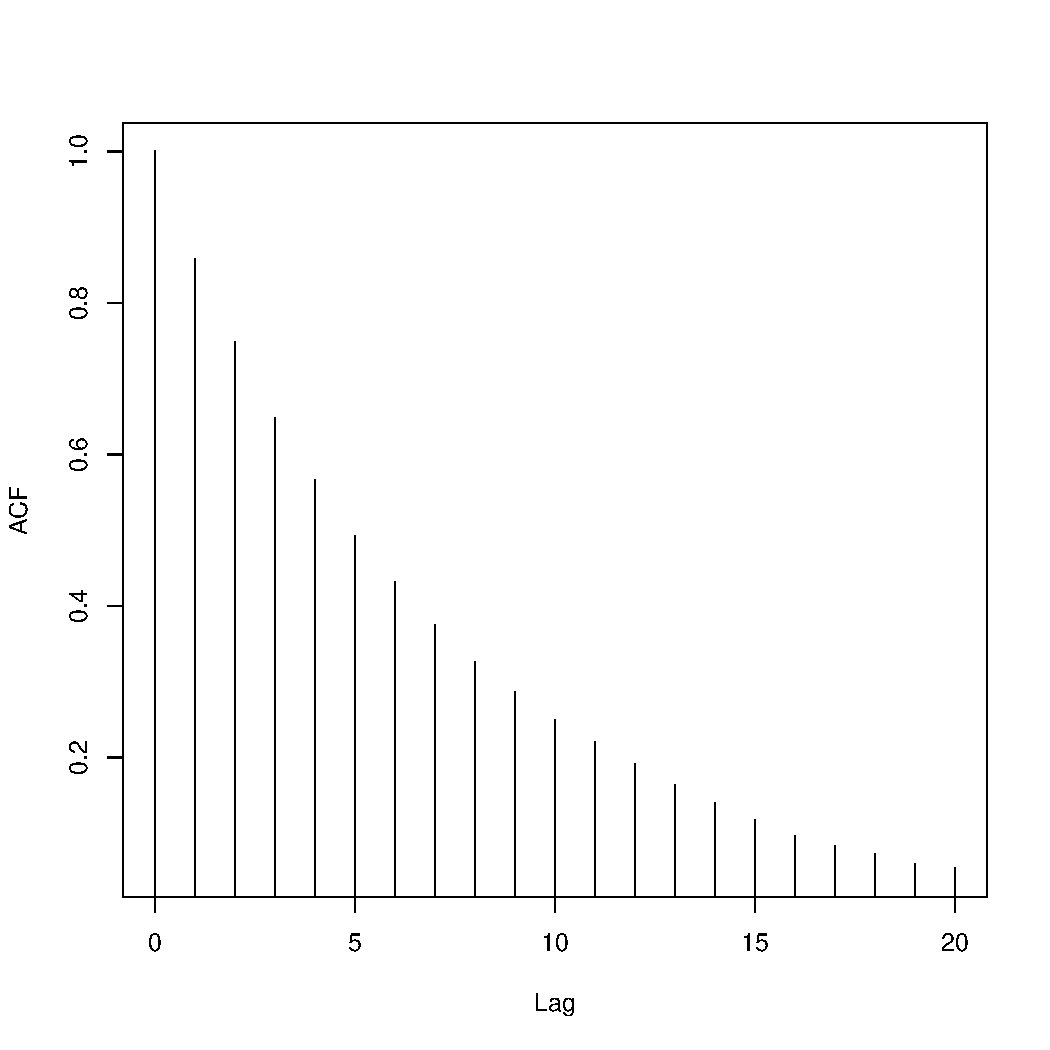
\includegraphics[width=80mm]{acf}
\caption{MCMCサンプルの自己相関関数}
\label{fig1}
\end{center}
\end{figure}
これを考慮し, 間引き数$15$としてMCMCサンプルを間引く.
最初に発生させるMCMCサンプルは$15500$個, バーンイン期間を$500$とし, 最終的には$1000$個のサンプルから事後期待値を計算する.

\subsection{結果}

比較対象の最尤推定での結果も合わせてMRE, MSEの様子を調べた結果, 図\ref{fig2}のようになった.
\begin{figure}[ht]
\begin{center}
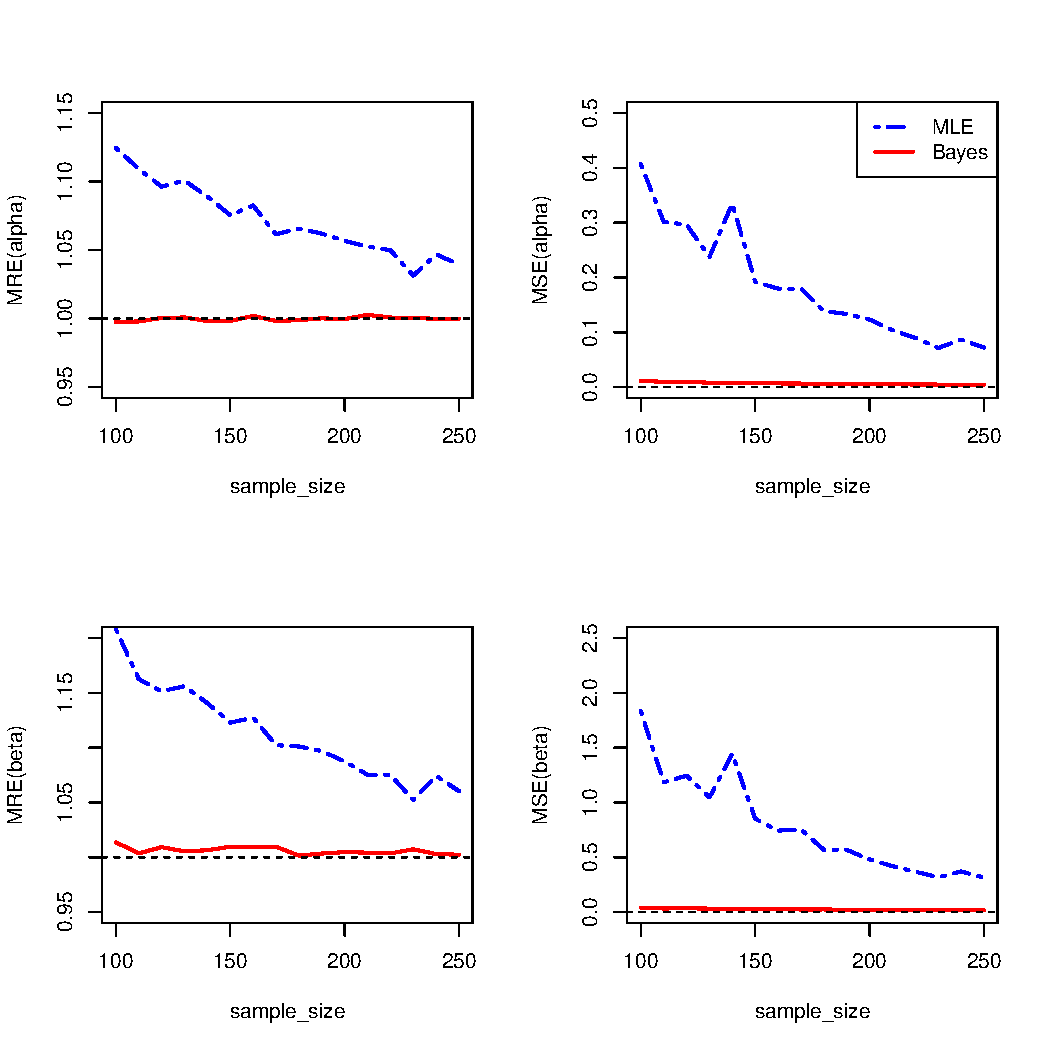
\includegraphics[width=120mm]{result}
\caption{シミュレーションの結果}
\label{fig2}
\end{center}
\end{figure}
最尤推定よりもベイズ推定の方が精度が優れているという結果となった.

\section{パラメータ\texorpdfstring{$\lambda_i$}について}

\subsection{5章の問題点}

\ref{sec_analysis}章のシミュレーションには問題点がある.
パラメータ$\lambda_i~(i=1,2,\ldots,n)$は\ref{definition}章にあるようにGamma$(\alpha,1)$に従う確率変数であるが, $\alpha $は未知であるためこの確率変数の実現値を得ることができない. そこで, 2つの提案を考えシミュレーションを行った.

\subsection{提案1}\label{suggestion1}
まずは$\lambda_i $を推定に用いずにパラメータの事後期待値を求めることを考える.

Jeffreysの事前分布を用いたとき, $\beta,\alpha$の同時事後分布は
$$
\pi(\beta ,\alpha |\bm{x})
\propto
\frac{\alpha^{n-1/2}\beta ^{-(n+1)}}{(\alpha +1)(\alpha +2)^{1/2}}
\prod_{i=1}^{n}
\left(1+\frac{x_{i}}{\beta }
\right)^{-(\alpha +1)}
$$
であった. これを用いて$2$変数のメトロポリス法により事後分布を求める.
それぞれのMCMCサンプルの自己相関関数は図\ref{fig3}のようになった. 
\begin{figure}[ht]
\begin{center}
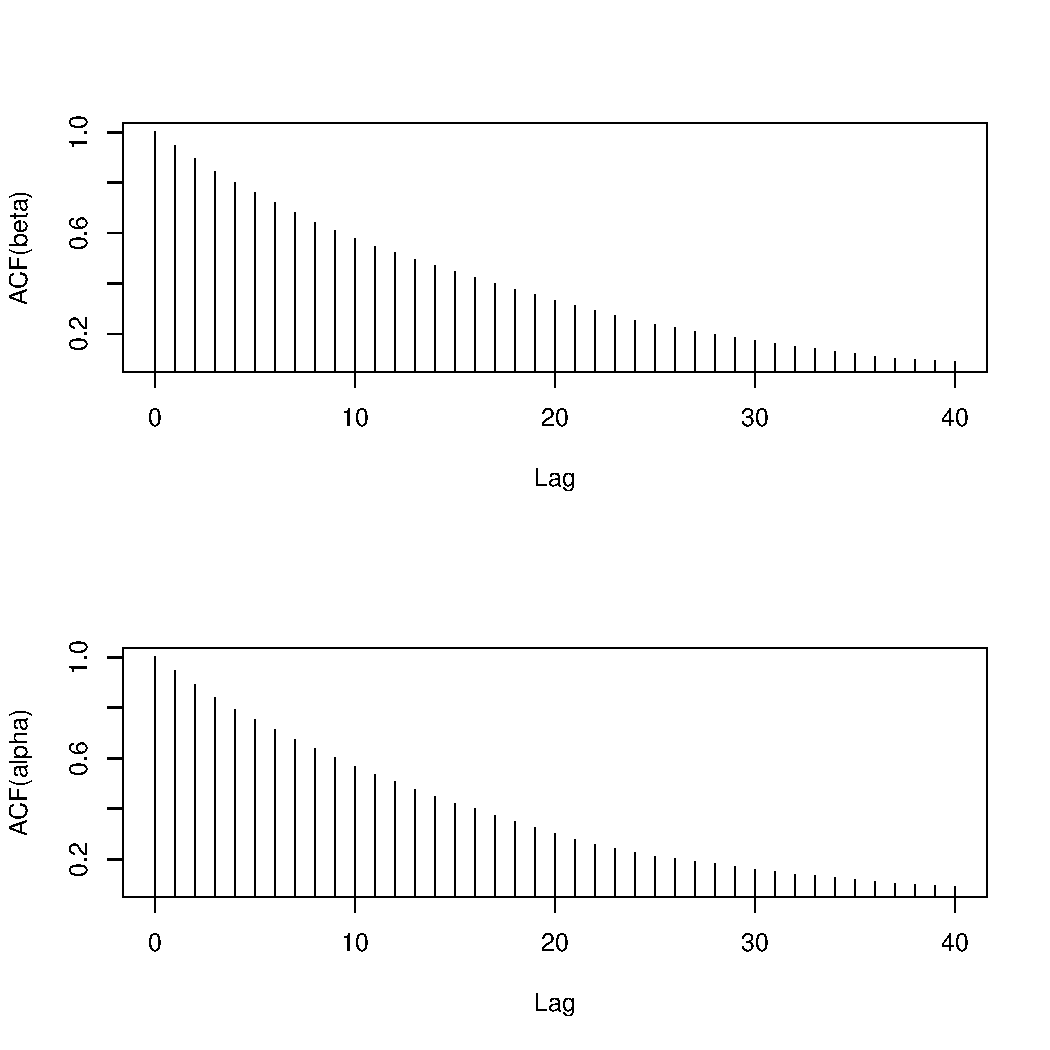
\includegraphics[width=100mm]{acf_notlambda}
\caption{提案1のMCMCサンプルの自己相関関数}
\label{fig3}
\end{center}
\end{figure}
これを考慮し, 間引き数を$30$としてMCMCサンプルを間引く. これに伴って最初に発生させるMCMCサンプルの数を増やし$31000$個とする. バーンイン期間を$1000$とし, 最終的に$1000$個のサンプルで事後分布を計算する. 結果は図\ref{fig4}のようになった.
\begin{figure}[ht]
\begin{center}
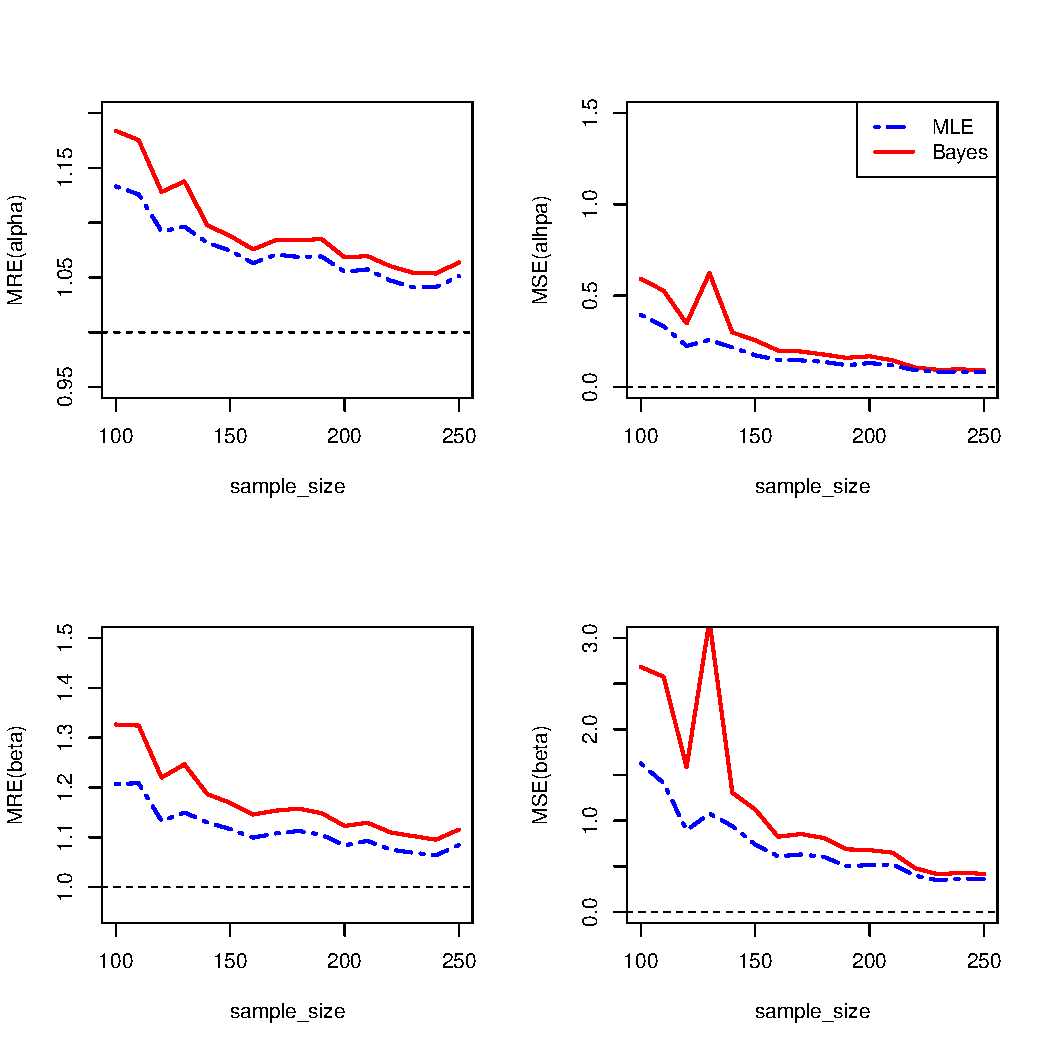
\includegraphics[width=120mm]{notlambda}
\caption{提案1の推定の結果}
 \label{fig4}
 \end{center}
\end{figure}
$\lambda_i$を用いずにメトロポリス法によって事後期待値を計算した場合, 最尤推定と比べて精度が低下した.

\subsection{提案2}\label{suggestion2}

次に, $\lambda_i$を推定し, その値を用いて$\beta,~\alpha$を推定する方法を考える.

サンプル$\bm{x}$が与えられた時の$\lambda_i$の条件付き分布は
$$
\lambda _{i}|x_i,\beta ,\alpha 
\sim 
\mbox{Gamma} \left(\alpha +1,1+\frac{x_{i}}{\beta }\right)
$$
であった.
これを最尤推定値$\hat{\beta },~\hat{\alpha }$を用いて
$$
\lambda _{i}|x_i,\hat{\beta } ,\hat{\alpha } 
\sim 
\mbox{Gamma} \left(\hat{\alpha } +1,1+\frac{x_{i}}{\hat{\beta }}\right)
$$
として各$\lambda_i$を推定する. そこからさらに\ref{sec_analysis}章の方法により$\beta ,\alpha $を推定し, 最尤推定値と精度を比較する. 
MCMCサンプルの自己相関関数は図\ref{fig5}のようになった.
\begin{figure}[ht]
\begin{center}
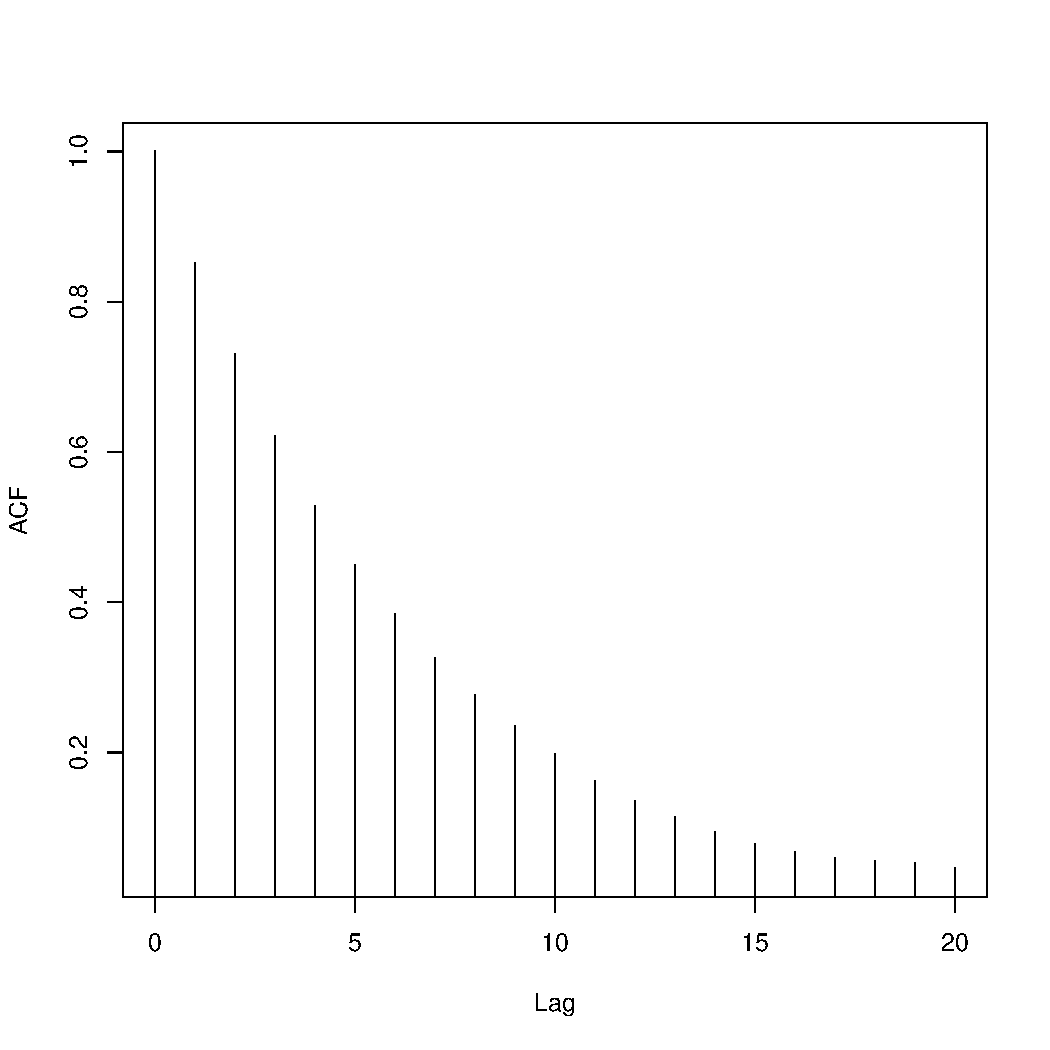
\includegraphics[width=80mm]{acf_mle-bayes}
\caption{提案2のMCMCサンプルの自己相関関数}
\label{fig5}
\end{center}
\end{figure}
自己相関関数は\ref{sec_analysis}章の方法と似た様子であるため, 同様に間引き数を$15$とし, 最初に発生させるMCMCサンプルの数を$15500$個, バーンイン期間を$500$とした.
結果は図\ref{fig6}のようになった.
\begin{figure}[ht]
\begin{center}
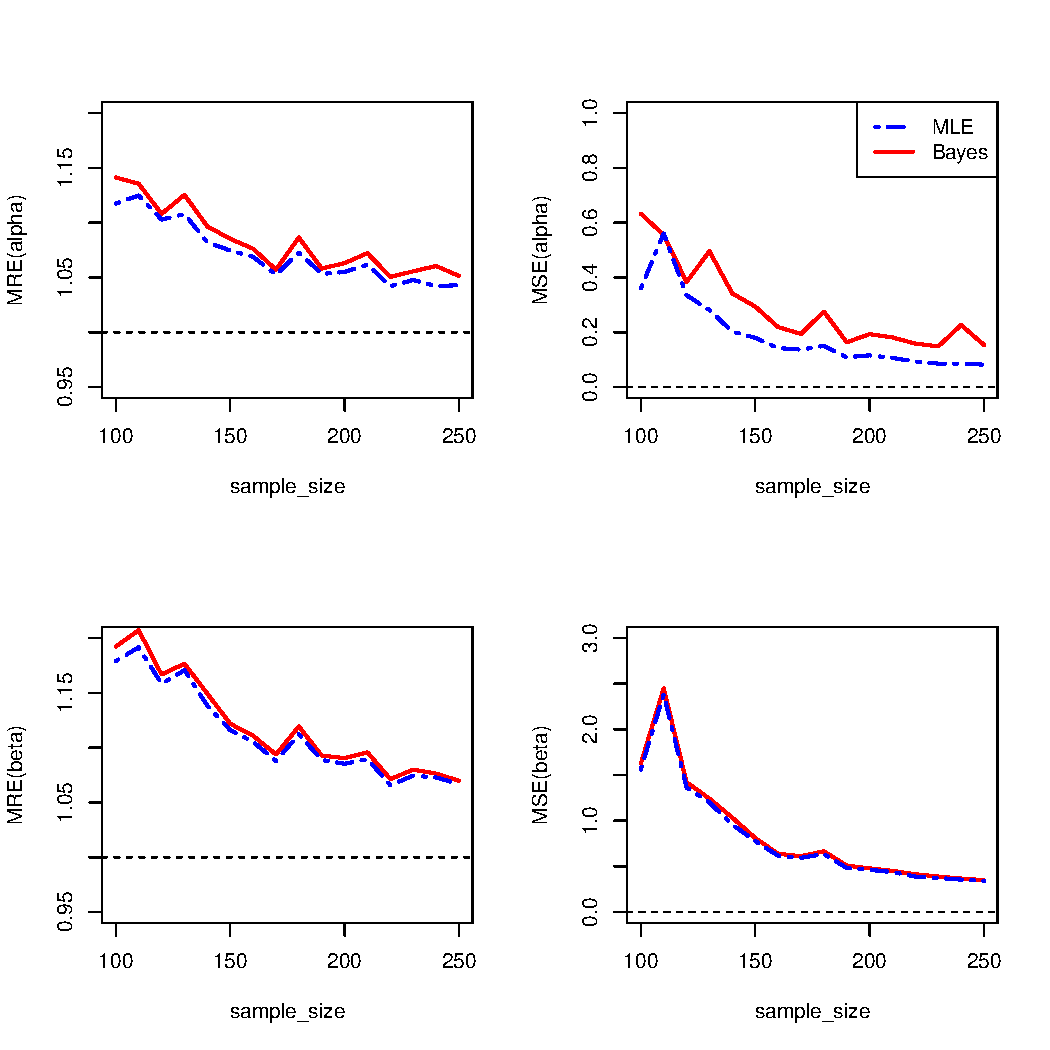
\includegraphics[width=120mm]{mle-bayes}
\caption{提案2の推定の結果}
\label{fig6}
\end{center}
\end{figure}
こちらの場合も最尤推定よりも優れた精度にはならなかった.

\section{まとめ}

\cite{Lomax2020}のシミュレーションの再現ではベイズ推定の方が精度が良いことが確認できたが, パラメータ$\lambda_i$が真のパラメータ$\alpha$によって定まる分布からの確率変数であり, 推定には用いることができないと考えられるため, 他の手法で推定を行うことができないかを検討した. 今回提案した二つの手法は$\lambda_i$を使わない方法と, $\lambda_i$を推定してから$\beta,\alpha$を推定する方法であるため, 現実的に用いることは可能であるが, 推定の精度は最尤推定より劣っていて, 実用的な手法を得ることはできなかった. 今後は$\lambda_i$を別の方法で生成, または$\lambda_i$を使わない方法によってより精度の高い推定法を考えることが課題である.

\section{シミュレーションに用いたRプログラム}

\ref{sec_analysis}章のプログラム

\begin{verbatim}
library("univariateML")
library("extraDistr")

true_beta = 2
true_alpha = 1.5

Metropolis <- function(current) {
  propose <- abs(rnorm(1,current,1))
  postOdds <- post_alpha(propose) / post_alpha(current)
  if(is.nan(postOdds)) current
  else if(min(postOdds,1) > runif(1,0,1)) propose else current
}

sample_size <- seq(100,250,by = 10)

bayes_mre_alpha_all <- c()
bayes_mse_alpha_all <- c()

bayes_mre_beta_all <- c()
bayes_mse_beta_all <- c()

MLE_mre_alpha_all <- c()
MLE_mse_alpha_all <- c()

MLE_mre_beta_all <- c()
MLE_mse_beta_all <- c()


for (n in sample_size){
  N = 1000 #1種類のサンプル数につき N回実験して平均を取る
  
  bayes_mres_alpha <- c()
  bayes_mses_alpha <- c()
  
  bayes_mres_beta <- c()
  bayes_mses_beta <- c()
  
  MLE_mres_alpha <- c()
  MLE_mses_alpha <- c()
  
  MLE_mres_beta <- c()
  MLE_mses_beta <- c()
  
  for (j in 1:N){
    x_total <- c()
    l_total <- c()
    
    #Lomaxに従う確率変数をn個生成
    for (k in 1:n){ 
      l <- rgamma(1,true_alpha,1)
      x <- rexp(1,l/true_beta)
      x_total <- append(x_total,x)
      l_total <- append(l_total,l)
    }
    
    post_alpha <- 
      function(alpha) 
        (1/((alpha + 1)*alpha^(1/2)*(alpha + 2)^(1/2)*(gamma(alpha))^n))*
        (prod(l_total))^(alpha - 1)
    
    
    nsteps <- 15500 #mcmcサンプリングの数
    alpha_mcmcsample <- rep(0,nsteps) #サンプルを格納するベクトル
    alpha_mcmcsample[1] <- 5 #初期値
    burn_in <- 500 
    
    for (i in 1:nsteps){
      alpha_mcmcsample[i+1] <- Metropolis(alpha_mcmcsample[i])
    }
    
    #burn_in
    alpha_mcmc_burned <- alpha_mcmcsample[-(1:burn_in)]
    length(alpha_mcmc_burned)
    
    #thin
    alpha_mcmc_thinned <- c()
    thin = 15
    for (i in 1:(nsteps-burn_in)){
      if(i%%thin == 0){
        alpha_mcmc_thinned <- append(alpha_mcmc_thinned, alpha_mcmc_burned[i])
      }
    }
    
    
    bayes_alpha_estimated <- mean(alpha_mcmc_thinned)
    bayes_beta_estimated <- sum(x_total*l_total)/(n-1)
    MLE_beta <- 1/mllomax(x_total)[1]
    MLE_alpha <- mllomax(x_total)[2]
    
    
    bayes_mres_alpha <- 
    append(bayes_mres_alpha, bayes_alpha_estimated*(1/true_alpha))
    bayes_mses_alpha <- 
    append(bayes_mses_alpha, (bayes_alpha_estimated - true_alpha)^2)
    
    bayes_mres_beta <- 
    append(bayes_mres_beta, bayes_beta_estimated*(1/true_beta))
    bayes_mses_beta <- 
    append(bayes_mses_beta, (bayes_beta_estimated - true_beta)^2)
    
    MLE_mres_alpha <- 
    append(MLE_mres_alpha, MLE_alpha*(1/true_alpha))
    MLE_mses_alpha <- 
    append(MLE_mses_alpha, (MLE_alpha - true_alpha)^2)
    
    MLE_mres_beta <- 
    append(MLE_mres_beta, MLE_beta*(1/true_beta))
    MLE_mses_beta <- 
    append(MLE_mses_beta, (MLE_beta - true_beta)^2)
    
  }
  bayes_mre_alpha_all <- 
  append(bayes_mre_alpha_all, (1/N)*sum(bayes_mres_alpha))
  bayes_mse_alpha_all <- 
  append(bayes_mse_alpha_all, (1/N)*sum(bayes_mses_alpha))
  
  bayes_mre_beta_all <- 
  append(bayes_mre_beta_all, (1/N)*sum(bayes_mres_beta))
  bayes_mse_beta_all <- 
  append(bayes_mse_beta_all, (1/N)*sum(bayes_mses_beta))
  
  MLE_mre_alpha_all <- 
  append(MLE_mre_alpha_all, (1/N)*sum(MLE_mres_alpha))
  MLE_mse_alpha_all <- 
  append(MLE_mse_alpha_all, (1/N)*sum(MLE_mses_alpha))
  
  MLE_mre_beta_all <- 
  append(MLE_mre_beta_all,(1/N)*sum(MLE_mres_beta))
  MLE_mse_beta_all <- 
  append(MLE_mse_beta_all,(1/N)*sum(MLE_mses_beta))
}

pdf("result.pdf")
par(mfrow=c(2,2)) 
plot(sample_size, bayes_mre_alpha_all, ylim = c(0.95, 1.15), ylab = "", 
type="l", lwd = 2, col = "red")
par(new=T)
plot(sample_size, MLE_mre_alpha_all, ylim = c(0.95, 1.15), ylab = "MRE(alpha)",
lty=6, type="l", lwd = 2, col = "blue")
abline(h=1,lty=2)

plot(sample_size, bayes_mse_alpha_all, ylim = c(0.0, 0.5), ylab = "", 
type="l", lwd = 2, col = "red")
par(new=T)
plot(sample_size, MLE_mse_alpha_all, ylim = c(0.0, 0.5), ylab = "MSE(alpha)", 
lty=6, type="l", lwd = 2, col = "blue")
abline(h=0,lty=2)
legend("topright", legend=c("MLE","Bayes"), 
lty=c(6,1),lwd = 2, col=c("blue","red"))

plot(sample_size, bayes_mre_beta_all, ylim = c(0.95, 1.2),  ylab = "", 
type="l", lwd = 2, col = "red") 
par(new=T)
plot(sample_size, MLE_mre_beta_all, ylim = c(0.95, 1.2),  ylab = "MRE(beta)", 
lty=6, type="l", lwd = 2, col = "blue")
abline(h=1,lty=2)

plot(sample_size, bayes_mse_beta_all, ylim = c(0.0, 2.5), ylab = "", 
type="l", lwd = 2, col = "red")
par(new=T)
plot(sample_size, MLE_mse_beta_all, ylim = c(0.0, 2.5),  ylab = "MSE(beta)", 
lty=6, type="l", lwd = 2, col = "blue")
abline(h=0,lty=2)
dev.off()

\end{verbatim}




\ref{suggestion1}のプログラム

\begin{verbatim}
library("univariateML")
library("extraDistr")

true_beta = 2
true_alpha = 1.5

sample_size <- seq(100,250,by = 10)

bayes_mre_alpha_all <- c()
bayes_mse_alpha_all <- c()

bayes_mre_beta_all <- c()
bayes_mse_beta_all <- c()

MLE_mre_alpha_all <- c()
MLE_mse_alpha_all <- c()

MLE_mre_beta_all <- c()
MLE_mse_beta_all <- c()



for (n in sample_size){
  #1種類のサンプル数につき N回実験して平均を取る
  N = 1000
  bayes_mres_alpha <- c()
  bayes_mses_alpha <- c()
  
  bayes_mres_beta <- c()
  bayes_mses_beta <- c()
  
  MLE_mres_alpha <- c()
  MLE_mses_alpha <- c()
  
  MLE_mres_beta <- c()
  MLE_mses_beta <- c()
  
  for (j in 1:N){
    x_total <- c()
    
    #Lomaxに従う確率変数をn個生成
    for (k in 1:n){
      l <- rgamma(1,true_alpha,1)
      x <- rexp(1,l/true_beta)
      x_total <- append(x_total,x)
    }
    
    post <- #事後分布
      function(beta, alpha) 
        ((alpha^(n-1/2))*beta^(-n-1))/((alpha + 1)*(alpha + 2)^(1/2))*
        (prod(1+x_total/beta))^(-(alpha + 1))
    
    nsteps <- 31000 #mcmcサンプリングの数
    beta_mcmc <- rep(0,nsteps) 
    alpha_mcmc <- rep(0,nsteps)
    beta_mcmc[1] <- 5
    alpha_mcmc[1] <- 5
    burn_in <- 1000
    
    
    for (i in 1:(nsteps-1)){
      propose_beta <- abs(rnorm(1,beta_mcmc[i],1))
      propose_alpha <- abs(rnorm(1,alpha_mcmc[i],1))
      postOdds <- 
      post(propose_beta, propose_alpha) / post(beta_mcmc[i], alpha_mcmc[i])
      if(is.nan(postOdds)){
        beta_mcmc[i+1] <- beta_mcmc[i]
        alpha_mcmc[i+1] <- alpha_mcmc[i]
      }
      else if(min(postOdds,1) > runif(1,0,1)){
        beta_mcmc[i+1] <- propose_beta
        alpha_mcmc[i+1] <- propose_alpha
      }else {
        beta_mcmc[i+1] <- beta_mcmc[i]
        alpha_mcmc[i+1] <- alpha_mcmc[i]
      }
    }
    
    
    #burn-in
    burned_beta <- beta_mcmc[-(1:burn_in)]
    burned_alpha <- alpha_mcmc[-(1:burn_in)]
    length(burned_beta)
    length(burned_alpha)
    
    #thin
    thinned_beta <- c()
    thinned_alpha <- c()
    
    for (i in 1:(nsteps-burn_in)){
      if(i%%10 == 0){
        thinned_beta <- append(thinned_beta, burned_beta[i])
        thinned_alpha <- append(thinned_alpha, burned_alpha[i])
      }
    }
    
    bayes_beta_estimated <- mean(thinned_beta)
    bayes_alpha_estimated <- mean(thinned_alpha)	
    MLE_beta <- 1/mllomax(x_total)[1]
    MLE_alpha <- mllomax(x_total)[2]
    
    bayes_mres_alpha <- 
    append(bayes_mres_alpha, bayes_alpha_estimated*(1/true_alpha))
    bayes_mses_alpha <- 
    append(bayes_mses_alpha, (bayes_alpha_estimated - true_alpha)^2)
    
    bayes_mres_beta <- 
    append(bayes_mres_beta, bayes_beta_estimated*(1/true_beta))
    bayes_mses_beta <- 
    append(bayes_mses_beta, (bayes_beta_estimated - true_beta)^2)
    
    MLE_mres_alpha <- 
    append(MLE_mres_alpha, MLE_alpha*(1/true_alpha))
    MLE_mses_alpha <- 
    append(MLE_mses_alpha, (MLE_alpha - true_alpha)^2)
    
    MLE_mres_beta <- 
    append(MLE_mres_beta, MLE_beta*(1/true_beta))
    MLE_mses_beta <- 
    append(MLE_mses_beta, (MLE_beta - true_beta)^2)
    
  }
  bayes_mre_alpha_all <- 
  append(bayes_mre_alpha_all, (1/N)*sum(bayes_mres_alpha))
  bayes_mse_alpha_all <- 
  append(bayes_mse_alpha_all, (1/N)*sum(bayes_mses_alpha))
  
  bayes_mre_beta_all <- 
  append(bayes_mre_beta_all, (1/N)*sum(bayes_mres_beta))
  bayes_mse_beta_all <- 
  append(bayes_mse_beta_all, (1/N)*sum(bayes_mses_beta))
  
  MLE_mre_alpha_all <- 
  append(MLE_mre_alpha_all, (1/N)*sum(MLE_mres_alpha))
  MLE_mse_alpha_all <- 
  append(MLE_mse_alpha_all, (1/N)*sum(MLE_mses_alpha))
  
  MLE_mre_beta_all <- 
  append(MLE_mre_beta_all,(1/N)*sum(MLE_mres_beta))
  MLE_mse_beta_all <- 
  append(MLE_mse_beta_all,(1/N)*sum(MLE_mses_beta))
}

pdf("notlambda.pdf")
par(mfrow=c(2,2)) 
plot(sample_size, bayes_mre_alpha_all, ylim = c(0.95, 1.2), ylab = "", 
type="l", lwd = 2, col = "red")
par(new=T)
plot(sample_size, MLE_mre_alpha_all, ylim = c(0.95, 1.2), ylab = "MRE(alpha)",
lty=6, type="l", lwd = 2, col = "blue")
abline(h=1, lty=2)

plot(sample_size, bayes_mse_alpha_all,ylim = c(0, 1.5), ylab = "", 
type="l", lwd = 2, col = "red") 
par(new=T)
plot(sample_size, MLE_mse_alpha_all,ylim = c(0, 1.5), ylab = "MSE(alhpa)", 
lty=6, type="l", lwd = 2, col = "blue")
abline(h=0, lty=2)
legend("topright", legend=c("MLE","Bayes"), 
lty=c(6,1), lwd = 2, col=c("blue","red"))

plot(sample_size, bayes_mre_beta_all, ylim = c(0.95, 1.5), ylab = "", 
type="l", lwd = 2, col = "red") 
par(new=T)
plot(sample_size, MLE_mre_beta_all, ylim = c(0.95, 1.5), ylab = "MRE(beta)", 
lty=6, type="l", lwd = 2, col = "blue")
abline(h=1, lty=2)

plot(sample_size, bayes_mse_beta_all, ylim = c(0, 3.0), ylab = "", 
type="l", lwd = 2, col = "red")
par(new=T)
plot(sample_size, MLE_mse_beta_all, ylim = c(0, 3.0), ylab = "MSE(beta)", 
lty=6, type="l", lwd = 2, col = "blue")
abline(h=0, lty=2)
dev.off()
\end{verbatim}



\ref{suggestion2}のプログラム

\begin{verbatim}
library("univariateML")
library("extraDistr")

true_beta = 2
true_alpha = 1.5

Metropolis <- function(current) {
  propose <- abs(rnorm(1,current,1))
  postOdds <- post_alpha(propose) / post_alpha(current)
  if(is.nan(postOdds)) current
  else if(min(postOdds,1) > runif(1,0,1)) propose 
  else current
}

sample_size <- seq(100,250,by = 10)

bayes_mre_alpha_all <- c()
bayes_mse_alpha_all <- c()

bayes_mre_beta_all <- c()
bayes_mse_beta_all <- c()

MLE_mre_alpha_all <- c()
MLE_mse_alpha_all <- c()

MLE_mre_beta_all <- c()
MLE_mse_beta_all <- c()



for (n in sample_size){
  #1種類のサンプル数につき N回実験して平均を取る
  N = 1000
  
  bayes_mres_alpha <- c()
  bayes_mses_alpha <- c()
  
  bayes_mres_beta <- c()
  bayes_mses_beta <- c()
  
  MLE_mres_alpha <- c()
  MLE_mses_alpha <- c()
  
  MLE_mres_beta <- c()
  MLE_mses_beta <- c()
  
  for (j in 1:N){
    x_total <- c()
    #l_total <- c()
    lambdas <- c()
    
    #Lomaxに従う確率変数をn個生成
    for (k in 1:n){
      l <- rgamma(1,true_alpha,1)
      x <- rexp(1,l/true_beta)
      x_total <- append(x_total,x)
    }
    
    #最尤推定の結果
    MLE_alpha <- mllomax(x_total)[2]
    MLE_beta <- 1/mllomax(x_total)[1]
    
    for (i in 1:n){
      lambdas[i] <- rgamma(1, MLE_alpha + 1, 1 + x_total[i]/MLE_beta)
    }
    
    #alphaの事後分布
    post_alpha <- 
      function(alpha) 
        (1/((alpha+1)*alpha^(1/2)*(alpha+2)^(1/2)*(gamma(alpha))^n))*
        (prod(lambdas))^(alpha - 1)
    
    
    nsteps <- 15500 #mcmcサンプリングの数
    alpha_mcmcsample <- rep(0,nsteps) #サンプルを格納するベクトル
    alpha_mcmcsample[1] <- 5 #初期値
    burn_in <- 500 
    
    for (i in 1:nsteps){
      alpha_mcmcsample[i+1] <- Metropolis(alpha_mcmcsample[i])
    }
    
    #burn-in
    alpha_mcmc_burned <- alpha_mcmcsample[-(1:burn_in)]
    length(alpha_mcmc_burned)
    
    #thin
    alpha_mcmc_thinned <- c()
    thin = 15
    for (i in 1:(nsteps-burn_in)){
      if(i%%thin == 0){
        alpha_mcmc_thinned <- append(alpha_mcmc_thinned, alpha_mcmc_burned[i])
      }
    }
    
    #ベイズ推定値
    bayes_alpha_estimated <- mean(alpha_mcmc_thinned)
    bayes_beta_estimated <- sum(x_total*lambdas)/(n-1)

    
    bayes_mres_alpha <- 
    append(bayes_mres_alpha, bayes_alpha_estimated*(1/true_alpha))
    bayes_mses_alpha <- 
    append(bayes_mses_alpha, (bayes_alpha_estimated - true_alpha)^2)
    
    bayes_mres_beta <- 
    append(bayes_mres_beta, bayes_beta_estimated*(1/true_beta))
    bayes_mses_beta <- 
    append(bayes_mses_beta, (bayes_beta_estimated - true_beta)^2)
    
    MLE_mres_alpha <- 
    append(MLE_mres_alpha, MLE_alpha*(1/true_alpha))
    MLE_mses_alpha <- 
    append(MLE_mses_alpha, (MLE_alpha - true_alpha)^2)
    
    MLE_mres_beta <- 
    append(MLE_mres_beta, MLE_beta*(1/true_beta))
    MLE_mses_beta <- 
    append(MLE_mses_beta, (MLE_beta - true_beta)^2)
    
  }
  
  bayes_mre_alpha_all <- 
  append(bayes_mre_alpha_all, (1/N)*sum(bayes_mres_alpha))
  bayes_mse_alpha_all <- 
  append(bayes_mse_alpha_all, (1/N)*sum(bayes_mses_alpha))
  
  bayes_mre_beta_all <- 
  append(bayes_mre_beta_all, (1/N)*sum(bayes_mres_beta))
  bayes_mse_beta_all <- 
  append(bayes_mse_beta_all, (1/N)*sum(bayes_mses_beta))
  
  MLE_mre_alpha_all <- 
  append(MLE_mre_alpha_all, (1/N)*sum(MLE_mres_alpha))
  MLE_mse_alpha_all <- 
  append(MLE_mse_alpha_all, (1/N)*sum(MLE_mses_alpha))
  
  MLE_mre_beta_all <- 
  append(MLE_mre_beta_all,(1/N)*sum(MLE_mres_beta))
  MLE_mse_beta_all <- 
  append(MLE_mse_beta_all,(1/N)*sum(MLE_mses_beta))
}

pdf("mle-bayes.pdf")
par(mfrow=c(2,2))
plot(sample_size, bayes_mre_alpha_all, ylim = c(0.95, 1.2), ylab = "", 
type="l", lwd = 2, col = "red")
par(new=T)
plot(sample_size, MLE_mre_alpha_all, ylim = c(0.95, 1.2), ylab = "MRE(alpha)",
lty=6, type="l", lwd = 2, col = "blue")
abline(h=1,lty=2)

plot(sample_size, bayes_mse_alpha_all, ylim = c(0.0, 1.0), ylab = "", 
type="l", lwd = 2, col = "red")
par(new=T)
plot(sample_size, MLE_mse_alpha_all, ylim = c(0.0, 1.0), ylab = "MSE(alpha)", 
lty=6, type="l", lwd = 2, col = "blue")
abline(h=0,lty=2)
legend("topright", legend=c("MLE","Bayes"), 
lty=c(6,1),  lwd = 2, col=c("blue","red"))

plot(sample_size, bayes_mre_beta_all, ylim = c(0.95, 1.2),  ylab = "", 
type="l", lwd = 2, col = "red") 
par(new=T)
plot(sample_size, MLE_mre_beta_all, ylim = c(0.95, 1.2),  ylab = "MRE(beta)", 
lty=6, type="l", lwd = 2, col = "blue")
abline(h=1,lty=2)

plot(sample_size, bayes_mse_beta_all, ylim = c(0.0, 3.0), ylab = "", 
type="l", lwd = 2, col = "red")
par(new=T)
plot(sample_size, MLE_mse_beta_all, ylim = c(0.0, 3.0),  ylab = "MSE(beta)", 
lty=6, type="l", lwd = 2, col = "blue")
abline(h=0,lty=2)
dev.off()
\end{verbatim}


\bibliographystyle{jplain}
\bibliography{sample,jsample}

\end{document}
